\chapter{加速器的验证和实验结果}

\section{加速器验证方法}

\subsection{}

\subsection{加速器功能验证}

\subsection{加速器性能验证}

\section{实验方法}


\section{实验结果}

\subsection{硬件属性}

\subsection{性能}

\subsection{能耗}

\subsection{讨论}

\subsubsection{熵编码和熵解码模块}
目前我们的加速器中并没有加入熵解码模块(entropy decoding module)来使得加速器支持权值熵编码,主要是考虑到熵解码模块需要耗费非常大的面积和能耗,但是仅仅能够获得非常有限的性能提升。一个熵解码模块(entropy decoding module)的面积为$6.781*10^{-3}mm^2$,它能够在一个cycle解码出一个码字。由于熵编码是一种变长编码,因此对应的解码模块必须串行进行解码。即使我们可以将数据划分为许多并行的数据流,然后对为每个数据流提供一个熵解码模块,这种方法将会引入巨大的面积和能耗开销。考虑到每一个SB需要在一个cycle提供$T_m\times 4$个数据,为了避免性能损失,我们必须为一个SB提供$T_m\times 4$个熵解码模块,因此我们在加速其中总共需要集成$T_n\times T_m\times 4$个熵解码模块。在$T_m = T_n = 16$的配置下,我们总共需要1024个熵解码模块,这将引入额外$6.94mm^2$的面积和$971.37mW$的功率,因此加速器的总面积和功率分别是$13.67mm^2$和$1769.92mW$,分别是原始设计的2.03倍和2.22倍。然而,新增熵解码的加速器在卷积层上几乎没有性能提升,在全连接层也只有1.18倍的性能提升,对比与额外的面积和功率开销,这种性能提升是非常有限的。因此,我们在加速器中不加入熵解码模块。

\subsubsection{稀疏度与性能}
\begin{figure}[h]
\centering
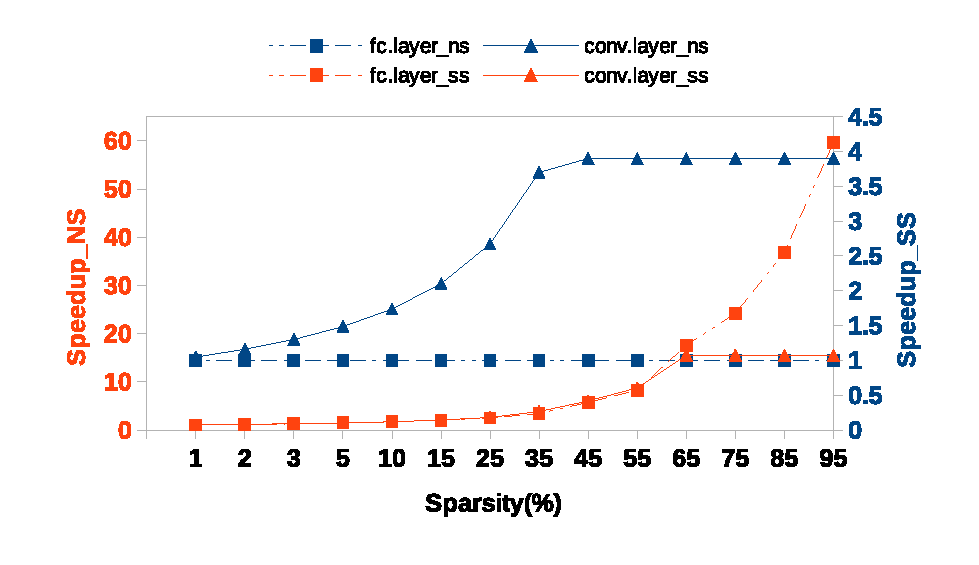
\includegraphics[width=1.0\columnwidth]{sensitivity.eps}
\caption{神经网络稀疏度对加速器性能的影响}
\label{fig:sensitivity}
\end{figure}



我们研究了加速器对神经网络稀疏度的敏感性,即稀疏度对神经网络性能的影响。如图~\ref{fig:sensitivity}所示,我们分别探究了神经元稀疏度和粗粒度权值稀疏度对加速器性能的影响,更进一步的,我们从卷积层和全连接层两个角度进行探究。从图中的数据我们观察到了几个有趣的实验结果:

1)考虑粗粒度权值稀疏,加速器能够在卷积层获得接近理想值的加速比(15.5倍 vs. 16倍)。为了兼容大多数网络的权值稀疏度~\ref{tab:sparsities},我们将NSM设计成为256选16的结构,即NSM最多从256个输入神经元中筛选出16个需要进行计算的神经元,从而最多实现16倍的加速器。我们的加速器能够接近理想加速器的主要原因是我们使用pingpong的模式管理片上缓存,使得加速器的片外访存延迟能够被运算时间覆盖。值得注意的是,由于我们的加速器能够充分利用粗粒度稀疏实现负载均衡,因此在相同稀疏度情况下,我们的加速器能够获得比Cambricon-X更优的加速比。

2)考虑粗粒度权值稀疏,在全连接层中,我们的加速器能够很容易地在低稀疏度情况下(低于$5\%$)获得加速比,并且随着稀疏度的提高,加速比也会不断提高,在稀疏度为$99\%$时能够获得59.59倍的加速比。主要原因是全连接层是一个访存密集的层,压缩后的权值能够大大减少片外访存数据量,从而减少片外访存时间,减少总执行时间。

3)考虑神经元稀疏,我们的加速器在卷积层最高能够获得3.9倍的加速比,接近理想的4倍加速比。由于在大多数情况下,神经元的稠密度高于$25\%$(稀疏度低于$75\%$),我们将SSM设计成为64选16的结构,因此最多获得4倍的加速比。这个设计能够满足绝大多数神经网络的需求。

4)


我们调查的稀疏敏感性加速器如图~ \ ref {无花果:敏感}我们不同神经元突触稀疏和粗粒度分别稀疏。我们做了几个有趣的观察。1)最大加速器的加速卷积层接近理想的加速(15.5美元\ * $和$ 16 \ * $)。兼容大部分神经网络(表~ \ ref {选项卡:稀疏}),销售经理设计选择16 256个神经元,从而实现最多16 \倍加速美元。我们的加速器达到近理想的加速通过隐藏背后的直接存储器存取内存访问的帮助下计算乒乓缓冲。值得注意的是,我们的加速器优于Cambricon-X突触在卷积层稀疏,作为我们的加速器可以充分利用数据重用和负载平衡从粗粒度的稀疏。
2)我们的加速器可以很容易地实现性能即使在稀疏只有95美元\ 20�全层,可以大大提高性能和降低稀疏(59.59美元\时报给稀疏的1美元\�。压缩突触大大减少内存访问时间,从而大大减少了总执行时间的全层。
    3)茂密的突触(

\subsubsection{减少的不规则度与性能}

\subsubsection{类似粗粒度稀疏的方法}

\subsubsection{其他稀疏神经网络加速器}

